\documentclass{article}

\usepackage{microtype}
\usepackage{graphicx}
\usepackage{booktabs}
\usepackage{tabularx}
\usepackage{array}
\usepackage{amsmath}
\usepackage{CJKutf8}
\usepackage{tikz}
\usepackage{icml2026}
\usepackage[capitalize,noabbrev]{cleveref}
\setcitestyle{numbers,square}
\usetikzlibrary{arrows.meta,positioning,shapes.geometric}
\newcommand{\zh}[1]{{\begin{CJK*}{UTF8}{bsmi}#1\end{CJK*}}}

\icmltitlerunning{Trustworthy Hybrid Workflows for Historical Script Translation}

\begin{document}

\twocolumn[
\icmltitle{Trustworthy AI for Cultural Heritage:\\ Conservative Hybrid Workflows for Endangered Historical Script Translation}

\begin{icmlauthorlist}
\icmlauthor{Anonymous Author}{anon}
\end{icmlauthorlist}

\icmlaffiliation{anon}{Anonymous Institution, Anonymous City, Anonymous Region, Anonymous Country}
\icmlcorrespondingauthor{Anonymous Author}{anon.email@domain.com}
\icmlkeywords{trustworthy AI, AI for good, cultural heritage, low-resource translation, historical scripts}

\vskip 0.3in
]

\printAffiliationsAndNotice{}

\begin{abstract}
Digital libraries, museum catalogs, and heritage archives are public information infrastructure, so historical-script translation errors can propagate as information-integrity failures rather than harmless model mistakes. We study this risk in ultra-low-resource Tangut title translation and a cross-script oracle-bone probe. Our workflow combines a strong dictionary-grounded frontier prompt, conservative local models that generate compact title candidates, and deterministic open selectors designed to avoid contamination and over-switching. On Tangut, the frontier baseline is the strongest single model (28.54 chrF++, 12/50 exact), but a simple open hybrid improves exact match to 13/50 with zero contamination, while a larger guarded open selector reaches 32.62 chrF++ without introducing contamination; a closed adjudicator is reported only as headroom. On a 200-item oracle-bone portability probe, a simple open 2-way selector improves the strongest single prompt baseline from 40/200 to 44/200 exact matches and reduces contamination from 3.5\% to 0.5\%. The main lesson for AI-for-good deployment is to privilege auditable candidate workflows and explicit failure containment over single-model wins.
\end{abstract}

\section{Introduction}

AI-for-good discussions often emphasize health, education, or civic applications, but cultural heritage is also a high-stakes public domain. Historical titles and catalog records flow into library systems, museum portals, teaching materials, and search interfaces that shape collective memory. In that setting, an apparently fluent but fabricated title is not just an NLP error: it is an information-integrity problem that can overwrite fragile evidence from endangered textual traditions.

Tangut short-title translation is a sharp instance of that problem. In the repository we study, only 491 real Tangut--Chinese pairs are available, and many references are compact catalog strings rather than ordinary sentences. Under such scarcity, a model can sound plausible while still producing the wrong historical title in the wrong form. Generic fluency-seeking objectives are therefore poorly matched to the real social requirement, which is conservative, auditable assistance for scholars and public-facing heritage institutions.

This changes the question we ask. The goal is not ``which model gets the best score on a tiny benchmark?'' Instead, once a strong frontier model is already available with dictionary grounding, what workflow remains trustworthy enough to use as a decision aid? We focus on three properties that matter for such use: low contamination, low over-expansion, and transparent switching behavior when a selector departs from the strongest single model.

The result is a workshop-style case study rather than a new architecture paper. We start from the strongest repository baseline: a DeepSeek v3.2 prompt with dictionary grounding and the exact later prompt family that outperformed the older local baseline prompt. We then test whether structured local models can contribute conservative alternatives, and whether open selectors can exploit those alternatives without opening new failure channels. Closed adjudication is retained only as headroom, not as the centerpiece.

The contribution to the workshop is therefore practical and deployment-oriented:
\begin{itemize}
    \item we frame endangered-script translation as trustworthy AI for public knowledge infrastructure, where contamination and fabricated normalization are the primary risks;
    \item we show that local learning is most useful when it produces conservative candidates that can be audited, rather than when it tries to replace the strongest frontier model end to end;
    \item we distill a small set of operational lessons for AI-for-good deployment under extreme scarcity: switch rarely, expose candidate provenance, and treat proprietary adjudication only as an upper bound.
\end{itemize}

\section{Setting, Stakes, and Trust Objectives}

\subsection{Why This Fits AI for Good}

The immediate application is preservation and access for endangered textual heritage. Better title reconstruction can help scholars, archivists, and the public search and compare materials that would otherwise remain opaque. But the same setting creates unusual downside risk: a wrong modernized title can become easier to reuse than the fragile original evidence it was meant to support. The system is therefore useful only if its failure modes are explicit and containable.

This places the task at the intersection of two workshop themes. First, it is an AI-for-social-good problem because it supports preservation of cultural memory under severe data scarcity. Second, it is an information-integrity problem because catalog errors can propagate through public institutions such as libraries and museums. Our design goal is not to maximize stylistic fluency, but to keep the model from smuggling unsupported content into records that may later be treated as authoritative.

\subsection{Task and Data}

The main benchmark is Tangut short-title translation into Chinese. The repository contains 491 real pairs, with 400 used for training and the remainder reserved for development and test. Because 400 examples are too few for ordinary fine-tuning, the local models are trained on 50k pseudo-parallel examples synthesized from historical Chinese and then mixed with 10x-upsampled real Tangut pairs, yielding 54k training rows per branch. The synthesis pipeline is dictionary-driven rather than opaque: a 24,133-entry Tangut lexicon induces a Chinese-to-Tangut map covering 3,353 Chinese characters, with 4.2 Tangut candidates per covered character on average. The targets are short historical titles, so exact form matters disproportionately.

All local branches share the same data budget and differ mainly in how they expose uncertainty. The simplest branches either leave misses explicit as \texttt{[UNK]} or expose them inside multitask alignment targets, while the more ambitious semantic-projection branch fills misses by vector-space nearest-neighbor lookup. In the stored 50k corpora, semantic projection removes explicit \texttt{[UNK]} tokens from the source side, but that apparent completeness does not yield a more trustworthy downstream model. This is why the workshop workflow privileges auditable MT-SFT candidates over silently projected inputs.

We also use a portability probe built from canonicalized oracle-bone readings mapped into the EVOBC inventory. This second benchmark is intentionally narrower than the Tangut task: it is a 200-item decipherment-style stress test rather than a matched short-title dataset. Its role is to test whether the conservative hybrid behavior transfers across scripts.

\subsection{Risk Model}

We operationalize trustworthiness through observable output risks rather than through a broad claim about ``safe AI.''

\paragraph{Contamination.} An output is flagged as contaminated iff it contains any Latin alphabetic character, angle-bracket markup, an explicit \texttt{[UNK]} token, or one of the prompt artifacts actually observed in stored runs, such as \texttt{assistant}, \texttt{manuals}, \texttt{networks}, or \texttt{shows}. The rule is deterministic and uses no tuned threshold.

\paragraph{Title-form errors.} We separately track truncation, over-expansion, and catalog-style slips such as suffix loss or numeral mismatch. These matter because a compact title can become unusable even when semantically related to the reference.

\paragraph{Over-switching.} A reranker that abandons the strongest single model too often is difficult to trust, even when its corpus overlap rises. On tiny datasets, switching frequency is itself a governance signal because it determines how many decisions a human would need to audit.

\paragraph{Evidence standard.} We report exact match, chrF++, contamination, and switching behavior directly in the main workshop version. A closed reference-aware judge remains useful background evidence, but the workshop claim is designed not to depend on it.

\begin{table}[t]
\centering
\small
\begin{tabularx}{\columnwidth}{@{}>{\raggedright\arraybackslash}p{0.23\columnwidth}>{\raggedright\arraybackslash}p{0.29\columnwidth}>{\raggedright\arraybackslash}X@{}}
\toprule
Risk & Why it matters for heritage systems & Workflow response \\
\midrule
Contamination & Prompt debris or mixed-script noise can pollute public records and search indexes. & Deterministic contamination flag plus conservative selectors that prefer clean title-form outputs. \\
Over-expansion & Fluent explanation can overwrite a compact canonical title with unsupported content. & Title-only prompting, local conservative candidates, and length-aware switching guards. \\
Over-switching & A selector that edits too often is hard for scholars to audit and can erase the strongest baseline's reliability. & Prefer low-switch open controls and report switch counts as a first-class metric. \\
Closed-model dependence & Opaque gains are hard to reproduce or institutionalize. & Use closed adjudication only as headroom; keep the main workflow claim on open selectors. \\
\bottomrule
\end{tabularx}
\caption{Risk framing for a scholar-facing decision aid. The workshop contribution is a workflow that makes these risks measurable and auditable.}
\label{tab:riskmap}
\end{table}

\section{Conservative Workflow Design}

\begin{figure}[t]
\centering
\resizebox{\columnwidth}{!}{%
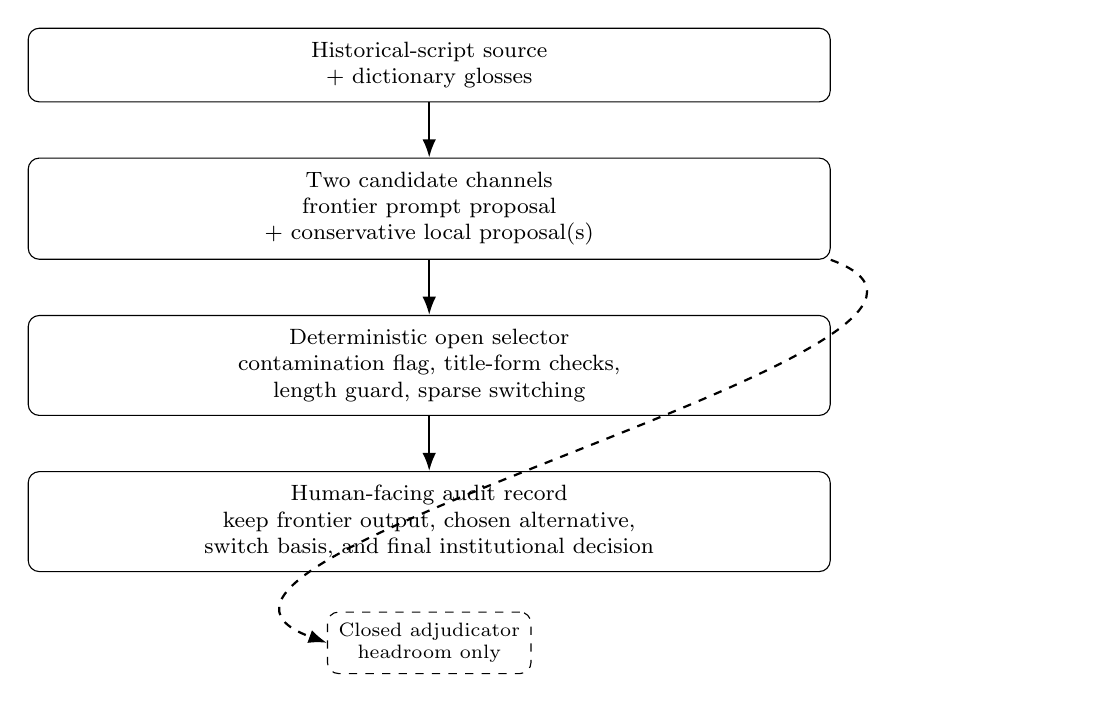
\begin{tikzpicture}[
    box/.style={draw, rounded corners, align=center, font=\footnotesize, minimum width=0.84\columnwidth, inner sep=5pt},
    side/.style={draw, dashed, rounded corners, align=center, font=\scriptsize, inner sep=4pt},
    arr/.style={-Latex, thick}
]
\node[box] (src) {Historical-script source \\ + dictionary glosses};
\node[box, below=7mm of src] (cands) {Two candidate channels \\ frontier prompt proposal \\ + conservative local proposal(s)};
\node[box, below=7mm of cands] (sel) {Deterministic open selector \\ contamination flag, title-form checks, \\ length guard, sparse switching};
\node[box, below=7mm of sel] (audit) {Human-facing audit record \\ keep frontier output, chosen alternative, \\ switch basis, and final institutional decision};
\node[side, below=5mm of audit] (closed) {Closed adjudicator \\ headroom only};
\draw[arr] (src) -- (cands);
\draw[arr] (cands) -- (sel);
\draw[arr] (sel) -- (audit);
\draw[arr, dashed] (cands.south east) to[out=-20,in=160] (closed.west);
\end{tikzpicture}
}
\caption{The proposed deployment posture. The main trustworthy-AI claim is not ``replace the frontier model,'' but ``preserve it, add conservative alternatives, and make switching auditable.''}
\label{fig:workflow}
\end{figure}

\paragraph{Strong frontier prompt.} The strongest single-model baseline uses \texttt{deepseek/deepseek-v3.2} through OpenRouter with dictionary grounding, four fixed development-set exemplars, temperature 0.0, a 512-token cap, and a title-only output constraint. This is the later prompt family that produced the strongest repository baseline, rather than the older local baseline prompt.

\paragraph{Structured local models.} Among the local learned systems, the most useful behavior comes from alignment-scaffolded multitask supervision. The local model is trained to emit dictionary matches, a literal draft, and the final compact title in one target string, which discourages premature free paraphrase. Notably, the more elaborate semantic-projection branch can hide uncertainty by removing explicit \texttt{[UNK]} from the synthetic source, but it still does not beat the simpler alignment-scaffolded design. For trustworthy deployment, hiding uncertainty was less useful than making it explicit and learnable.

\paragraph{Open selectors.} We evaluate deterministic open selectors over candidate pools containing the frontier output and one or more local outputs. The smallest selector is a guarded 2-way switcher over frontier plus MT-SFT. The larger open controls are plurality vote and a 3-way guarded selector over frontier, UNK-SFT, and gap-filtered MT-DPO. A proprietary 3-way adjudicator is reported only as headroom.

\paragraph{Prompt-matched local controls.} To avoid attributing the frontier advantage to prompt wording alone, we also rerun the exact DeepSeek-style few-shot prompt on local Qwen2.5-7B, with and without conservative lexical beam constraints. The chosen frontier prompt family is not arbitrary: on the shared 5-item pilot slice, the final few-shot title-only variant reached 2/5 exact matches and 67.68 chrF++, versus 0/5 and 21.99 for a stricter title-only prompt.

\Cref{fig:workflow} summarizes the intended use pattern. The selector is deliberately narrow: it does not rewrite candidates freely, and it should always leave behind an audit trail that records whether the frontier proposal was kept or replaced. This is the core workshop distinction between a benchmark-only reranker and a workflow that a public institution could plausibly inspect.

\section{Evidence}

\begin{table}[t]
\centering
\small
\begin{tabularx}{\columnwidth}{@{}>{\raggedright\arraybackslash}Xcccc@{}}
\toprule
System & Exact & chrF++ & Contam. & Switches \\
\midrule
Frontier DeepSeek & 12/50 & 28.54 & 0.0\% & -- \\
Local Qwen, same prompt & 1/50 & 12.18 & 6.0\% & -- \\
+ lexical beam & 1/50 & 12.35 & 8.0\% & -- \\
MT-SFT & 5/50 & 25.99 & 2.0\% & -- \\
Guarded 2-way (frontier + MT-SFT) & 13/50 & 30.05 & 0.0\% & 1 \\
Plurality 3-way (open) & 13/50 & 30.06 & 0.0\% & 2 \\
Guarded 3-way (open) & 12/50 & 32.62 & 0.0\% & 12 \\
Pairwise chrF-MBR (open) & 11/50 & 34.76 & 6.0\% & 35 \\
Closed 3-way adjudicator & 14/50 & 34.87 & 0.0\% & -- \\
\bottomrule
\end{tabularx}
\caption{Tangut headline systems. ``Switches'' counts how often a selector departs from the frontier output. The main workshop claim is carried by the open rows.}
\label{tab:tangut}
\end{table}

\paragraph{The strongest single model is still frontier prompting.}
\Cref{tab:tangut} starts from a deliberately strong baseline, because a trustworthy workflow should be judged against the best available single system rather than against a weak local prompt. That baseline reaches 12/50 exact matches with zero contamination. Matching the frontier prompt on local Qwen2.5-7B helps relative to the older local prompt, but remains weak at 1/50 exact. Adding lexical beam constraints changes little. This rules out a cheap explanation: the frontier advantage is not just prompt wording wrapped around the same local model.

\paragraph{Local learning matters mainly by generating conservative alternatives.}
MT-SFT does not beat the frontier system head to head, but it contributes a different error profile. In the stored diagnostics, frontier prompting is already clean but still exhibits one truncation and one over-expansion case; MT-SFT is weaker overall yet often more conservative on compact catalog strings. This is exactly the behavior a trustworthy hybrid needs: not a second system that always wins, but one that occasionally repairs frontier mistakes without adding visible artifacts.

\paragraph{Gap-filtered DPO is auxiliary, not foundational.}
The broader benchmark includes MT-DPO as a third candidate source, but the trustworthy reading of that result is narrow. Across the stored 3,867 preference pairs, the current reward is functionally lexical-coverage-driven: removing the weak $0.01 \log \mathrm{PPL}$ tie-breaker causes zero pair-order flips, while the high-confidence gap filter at $\ge 0.4$ retains only 498 pairs and raises a simple gold-proxy label-quality check from 71.3\% overall to 81.5\%. We therefore use MT-DPO only as an auxiliary candidate source in the larger pool, not as the foundation of the workshop claim.

\paragraph{Helpful open hybrids switch rarely.}
The guarded 2-way hybrid over frontier and MT-SFT improves exact match from 12/50 to 13/50 while staying at zero contamination, and it does so by switching only once. Plurality vote over a larger 3-way pool reaches the same exact-match gain with only two switches. This is the strongest trust signal in the Tangut benchmark: the useful open hybrids are conservative enough that a human reviewer could realistically inspect every switch.

\paragraph{More overlap is not the same as more trust.}
Pairwise chrF-MBR is the crucial negative control. It raises corpus chrF++ to 34.76, but it switches away from the frontier output on 35 of 50 items, introduces 6\% contamination, and drops exact match to 11/50. In this regime, agreement-seeking selection overshoots. The workshop lesson is that switching behavior itself must be treated as a trustworthiness variable, not just an implementation detail.

\begin{table}[t]
\centering
\small
\begin{tabularx}{\columnwidth}{@{}>{\raggedright\arraybackslash}Xcccc@{}}
\toprule
Method & Exact & Contam. & Suffix OK & Len. ratio \\
\midrule
Frontier DeepSeek & 12/50 & 0.0\% & 24/27 & 0.95 \\
Guarded 2-way & 13/50 & 0.0\% & 24/27 & 0.97 \\
Plurality 3-way & 13/50 & 0.0\% & 24/27 & 0.97 \\
Guarded 3-way & 12/50 & 0.0\% & 23/27 & 0.98 \\
Pairwise chrF-MBR & 11/50 & 6.0\% & 24/27 & 1.17 \\
\bottomrule
\end{tabularx}
\caption{Trust-aligned diagnostics for open selectors. Low-switch methods preserve title length and stay clean; MBR overshoots toward longer outputs.}
\label{tab:trustdiag}
\end{table}

\paragraph{Tangut evidence is directional rather than definitive.}
The Tangut test set contains only 50 items, so we avoid grand claims about statistical separation. Stored bootstrap analyses show overlapping exact-match intervals for frontier prompting (24\%, 95\% CI [12, 36]), plurality vote (26\%, [14, 38]), and the larger guarded 3-way selector (24\%, [12, 36]). The responsible claim is therefore not ``the open selector decisively wins,'' but that several independent open hybrids preserve cleanliness and occasionally recover extra correct titles, whereas aggressive MBR over-switches.

\begin{table}[t]
\centering
\scriptsize
\begin{tabularx}{\columnwidth}{@{}>{\raggedright\arraybackslash}p{0.18\columnwidth}>{\raggedright\arraybackslash}p{0.28\columnwidth}>{\raggedright\arraybackslash}p{0.28\columnwidth}>{\raggedright\arraybackslash}X@{}}
\toprule
Case & Reference & Candidate trace & Audit lesson \\
\midrule
Truncation repair & \zh{番言金剛王乘根} & F: \zh{番};\newline Open: \zh{番言金剛王乘根} & A rare switch can exactly repair an obvious truncation. \\
Contamination refusal & \zh{七寶華踏佛陀羅尼經} & F/Open: \zh{七寶花踏佛陀羅尼經};\newline MBR: \zh{七寶華嚴大羅}\texttt{Networked\hspace{0pt}Bronze}\zh{經} & Reject a contaminated candidate even when agreement is higher. \\
\bottomrule
\end{tabularx}
\caption{Two stored Tangut cases that anchor the trustworthiness claim.}
\label{tab:cases}
\end{table}

\Cref{tab:cases} makes the item-level behavior concrete. The useful intervention is narrow and auditable: one switch repairs an obvious truncation, while one refused switch blocks a visibly contaminated candidate from entering the final workflow.

\begin{table}[t]
\centering
\small
\begin{tabular}{lccc}
\toprule
System & Exact & chrF++ & Contam. \\
\midrule
Dict-grounded prompt & 40/200 & 46.20 & 3.5\% \\
MT-SFT \texttt{<literal>} & 29/200 & 40.56 & 5.0\% \\
Simple 2-way selector & 44/200 & 47.81 & 0.5\% \\
Best-of-2 oracle & 48/200 & 51.47 & 2.0\% \\
\bottomrule
\end{tabular}
\caption{Cross-script portability probe on canonicalized oracle-bone decipherment. The open selector improves the strongest single prompt baseline while sharply reducing contamination.}
\label{tab:evobc}
\end{table}

\paragraph{The portability probe repeats the same safety pattern.}
\Cref{tab:evobc} reports the 200-item oracle-bone probe. The strongest single system is again the dictionary-grounded prompt baseline, not the local model. But the same hybrid lesson survives transfer: a simple open 2-way selector improves exact match from 40/200 to 44/200 and reduces contamination from 3.5\% to 0.5\%. The probe is still format-mismatched relative to Tangut title translation, but it makes the workflow story harder to dismiss as a one-script accident.

\section{Workshop Lessons: From Benchmarks to Deployment Posture}

The main workshop takeaway is not a new state of the art; it is a deployment stance for high-risk, low-data historical NLP. When outputs may flow into public catalogs or archival interfaces, the safest design is not to trust one model's fluent answer. It is to preserve a strong frontier proposal, add a conservative local counterproposal, and expose the selector's decision in a form that humans can audit.

This suggests four operational rules for AI-for-good use in cultural heritage settings:
\begin{enumerate}
    \item \textbf{Keep the strongest baseline visible.} A selector should not erase the frontier proposal from the audit trail.
    \item \textbf{Switch only under narrow conditions.} Low switch counts are a feature, not a weakness, when each switch can be examined by a scholar or curator.
    \item \textbf{Treat contamination as a hard failure.} Artifact leakage is more damaging here than small lexical disagreement because it directly pollutes public records.
    \item \textbf{Use proprietary adjudication only as headroom.} Closed models may show how much complementarity remains, but an institutionally usable workflow should rest on components that can be rerun and inspected.
\end{enumerate}

This positioning is deliberately closer to trustworthy decision support than to automatic translation deployment. The system is useful because it narrows a human's review space and suppresses dangerous failure modes, not because it has reached scholar-replacing accuracy.

For public-institution use, this also implies a documentation norm. A library, archive, or museum should not ingest only the final string. It should preserve the source item, the frontier proposal, the local alternative when present, the selector's basis for switching, and any contamination flags. This is a lightweight but concrete governance requirement: if the workflow cannot explain why a title changed, it is not ready to support cataloging.

\section{Limitations}

The paper remains a constrained case study. The main Tangut test set is still only 50 items, so even honest gains are fragile. The oracle-bone probe is larger but format-mismatched; it tests cross-script portability of the workflow, not matched title translation. Some upstream ingredients are also still stronger in closed form, especially the frontier model itself and the closed 3-way adjudicator that we use only as headroom. Finally, this workshop version is intentionally not a scholar-in-the-loop deployment study. It narrows a trustworthy workflow family, but expert review is still required before any catalog curation or public-facing heritage tool should rely on the outputs.

\section*{Impact Statement}

The intended positive impact is improved access to endangered textual heritage with fewer hallucinated or contaminated translations entering digital catalogs. The main misuse risk is false scholarly authority: even a fluent system can produce persuasive but incorrect historical titles. For that reason, the paper emphasizes deterministic contamination checks, conservative open selectors, visible candidate provenance, and human verification rather than autonomous deployment.

\begin{thebibliography}{10}
\small

\bibitem{arthur2016lexicons}
Philip Arthur, Graham Neubig, and Satoshi Nakamura.
\newblock 2016.
\newblock Incorporating Discrete Translation Lexicons into Neural Machine Translation.
\newblock In \emph{Proceedings of EMNLP}.

\bibitem{domingo2018backtranslation}
Miguel Domingo and Francisco Casacuberta.
\newblock 2018.
\newblock A Machine Translation Approach for Modernizing Historical Documents Using Backtranslation.
\newblock In \emph{Proceedings of IWSLT}.

\bibitem{hokamp2017lexically}
Chris Hokamp and Qun Liu.
\newblock 2017.
\newblock Lexically Constrained Decoding for Sequence Generation Using Grid Beam Search.
\newblock In \emph{Proceedings of ACL}.

\bibitem{lu2024cod}
Hongyuan Lu et al.
\newblock 2024.
\newblock Chain-of-Dictionary Prompting Elicits Translation in Large Language Models.
\newblock In \emph{Proceedings of EMNLP}.

\bibitem{rafailov2023dpo}
Rafael Rafailov et al.
\newblock 2023.
\newblock Direct Preference Optimization: Your Language Model is Secretly a Reward Model.
\newblock In \emph{Proceedings of NeurIPS}.

\bibitem{sennrich2016monolingual}
Rico Sennrich, Barry Haddow, and Alexandra Birch.
\newblock 2016.
\newblock Improving Neural Machine Translation Models with Monolingual Data.
\newblock In \emph{Proceedings of ACL}.

\bibitem{sommerschield2023ancient}
Thea Sommerschield et al.
\newblock 2023.
\newblock Machine Learning for Ancient Languages: A Survey.
\newblock \emph{Computational Linguistics}, 49(3).

\bibitem{wang2023evahanoverview}
Wang et al.
\newblock 2023.
\newblock EvaHan2023: Overview of the First International Ancient Chinese Translation Bakeoff.
\newblock In \emph{Proceedings of ALT2023: Ancient Language Translation Workshop}.

\end{thebibliography}

\clearpage
\appendix
\onecolumn

\section{Reproducibility Details}

This appendix collects the operational details that were compressed in the workshop body. The main claim still rests on the open-selector results; the closed rows are kept only to document the frontier baseline and remaining headroom. Relative to the body, the appendix mainly adds three things: data provenance and hygiene, reward/judge robustness notes, and the concrete fields needed for institutional auditability.

\subsection{Open and Closed Components}

\begin{table}[H]
\centering
\small
\begin{tabular}{lll}
\toprule
Component & Status & Role \\
\midrule
DeepSeek v3.2 prompt baseline & closed & strongest single candidate source \\
MT-SFT / gap-filtered DPO & open/local & conservative alternative candidates \\
Plurality / guarded selectors & open & main workflow claim \\
Closed 3-way adjudicator & closed & upper bound only \\
\bottomrule
\end{tabular}
\caption{The workshop claim is intentionally placed on the open selector rows rather than on the closed adjudicator.}
\label{tab:openclosed}
\end{table}

\subsection{Synthetic Data Construction and Hygiene}

\begin{table}[H]
\centering
\small
\begin{tabular}{lc}
\toprule
Item & Value \\
\midrule
Dictionary entries & 24,133 \\
Covered Chinese characters & 3,353 \\
Avg. Tangut candidates / covered char & 4.2 \\
Synthetic rows per branch & 50,000 \\
Real-train upsampling & $400 \times 10 = 4,000$ \\
Combined rows per branch & 54,000 \\
Exact test overlap with train/dev/synth/few-shot & 0 \\
\bottomrule
\end{tabular}
\caption{Compact provenance and hygiene summary for the Tangut local-training pipeline.}
\label{tab:synthdata}
\end{table}

All local branches share the same sample budget and differ only in how missing Chinese characters are handled. \texttt{mixed} replaces roughly 30--70\% of dictionary hits with Tangut while leaving residual Chinese visible; \texttt{unk} makes every miss explicit as \texttt{[UNK]}; \texttt{semantic} uses top-3 FAISS retrieval with vote-based replacement and \texttt{[UNK]} fallback; \texttt{multitask} emits \texttt{<dict\_match>...</dict\_match> <literal>...</literal> final-title} targets. In the stored 50k corpora, the semantic branch contains zero explicit \texttt{[UNK]} source tokens, whereas the UNK and multitask branches expose 66,879 placeholder positions. The workflow therefore does not equate fewer visible unknowns with more trustworthy training data.

\subsection{Inference Settings and Selection Pools}

\begin{table}[H]
\centering
\small
\begin{tabularx}{\textwidth}{@{}l>{\raggedright\arraybackslash}X>{\raggedright\arraybackslash}X@{}}
\toprule
Component & Configuration & Why it matters \\
\midrule
Frontier prompt & \texttt{deepseek/deepseek-v3.2} via OpenRouter; four fixed development-set exemplars; dictionary grounding; temperature 0.0; max 512 output tokens; title-only output format & Strongest single candidate source and main closed baseline. \\
Prompt-matched local control & Local Qwen2.5-7B with the same DeepSeek-style few-shot prompt; optional conservative lexical beam & Diagnostic check that prompt wording alone does not explain the frontier gap. \\
Guarded 2-way open selector & Pool = \{frontier, MT-SFT\}; deterministic contamination flag; sparse-switch preference & Smallest fully open hybrid and main reproducible workflow claim on Tangut. \\
Guarded 3-way open selector & Pool = \{frontier, UNK-SFT, gap-filtered MT-DPO\}; contamination and title-form guards & Higher chrF++ but much more switching, so treated as a stress test rather than the default deployment path. \\
\bottomrule
\end{tabularx}
\caption{Compact operational settings for the main workflow components discussed in the workshop draft.}
\label{tab:settings}
\end{table}

\subsection{Frontier Prompt Note}

The frontier baseline is deterministic, so there is no sampling-seed variance to report. We also do not present a paid exhaustive prompt sweep as if it were free. What we can document is the stored pilot that motivated the final prompt family: on the shared 5-item slice, the final few-shot title-only prompt reaches 2/5 exact matches and 67.68 chrF++, whereas a stricter title-only variant reaches 0/5 and 21.99 chrF++. This is not a full robustness study, but it shows that the final prompt choice was evidence-based rather than arbitrary.

\subsection{Operational Contamination Definition}

An output is marked contaminated iff it contains at least one of the following:
\begin{itemize}
    \item any Latin alphabetic character;
    \item angle-bracket markup such as raw task tags;
    \item an explicit \texttt{[UNK]} token;
    \item one of the prompt-artifact lexemes actually observed in stored runs, including \texttt{assistant}, \texttt{manuals}, \texttt{networks}, or \texttt{shows}.
\end{itemize}

This definition is deterministic and threshold-free. In the Tangut results, the clean open selectors preserve the frontier model's zero-contamination regime, while pairwise chrF-MBR and weak local prompt controls do not.

\subsection{Deterministic Selector Logic}

The default open selector used in the workshop draft is the \texttt{guarded} mode from \texttt{experiments/open\_hybrid\_heuristic.py}. The 2-way and 3-way variants share the same logic; they differ only in candidate pool size. The exact contamination regex used by both the selector and the downstream audit scripts is:
\begin{quote}
\small\ttfamily
\verb+[A-Za-z<>]|\[UNK\]|assistant|manuals|networks|shows|grat|dresses+
\end{quote}

The selector also uses the explicit title-suffix set \zh{經論記疏頌儀義傳錄贊序字品文觀根次門}. For each candidate $y$ in a pool, it computes:
\[
\begin{aligned}
\mathrm{score}(y)=\;&1.4 \cdot \mathrm{prefix\_consensus}
 +1.2 \cdot \mathrm{suffix\_consensus}
 +2.5 \cdot \mathrm{has\_title\_suffix} \\
&-1.0 \cdot |\mathrm{len}(y)-\mathrm{median\_len}|
 -6.0 \cdot \mathrm{contamination}
 -4.0 \cdot \mathrm{too\_short} \\
&-2.0 \cdot \mathrm{too\_long}
 +0.75 \cdot \mathbf{1}[y=\mathrm{frontier}],
\end{aligned}
\]
where prefix/suffix consensus sums common-prefix/common-suffix lengths of at least 2 characters against the other candidates, \texttt{too\_short} means $\mathrm{len}(y) \le \max(1,\lfloor \mathrm{source\_len}/4 \rfloor)$, and \texttt{too\_long} means $\mathrm{len}(y) \ge \mathrm{median\_len}+5$ and $\mathrm{len}(y) \ge \mathrm{source\_len}+5$.

The default \texttt{guarded} decision rule is frontier-first:
\begin{enumerate}
    \item if the frontier candidate is contaminated and the best local candidate is clean, switch;
    \item if the frontier candidate has length $\le 1$ and the best local candidate has length $\ge 3$, switch;
    \item otherwise compute the best local candidate by score, and switch only if all of the following hold:
    \begin{itemize}
        \item local score margin over frontier $\ge 3.0$;
        \item local prefix+suffix consensus exceeds frontier consensus by at least 2;
        \item the local candidate is not contaminated and not too short;
        \item if the frontier ends with a title suffix, the local candidate must also end with a title suffix;
    \end{itemize}
    \item otherwise, if the frontier is flagged as too long, the local candidate is not too long, local consensus is at least 2, and the local candidate is at least 2 characters shorter, switch;
    \item else keep the frontier candidate.
\end{enumerate}

The \texttt{score\_max} ablation removes the guarded switch logic and simply returns the highest-scoring candidate. This is why it switches much more often in the sensitivity study and is reported only as a stress test rather than a deployment default.

\section{Additional Diagnostics}

The workshop body reports point estimates and a small set of trust-oriented metrics. The tables below keep the small-sample results interpretable by adding stored intervals and coarse error counts.

\subsection{Uncertainty Estimates}

\begin{table}[H]
\centering
\small
\begin{tabular}{llcc}
\toprule
Suite & Method & Exact (95\% CI) & chrF++ (95\% CI) \\
\midrule
Tangut & Frontier DeepSeek & 12/50 [14.3, 37.4]\% & 28.54 [20.87, 37.60] \\
Tangut & Plurality 3-way & 13/50 [14.0, 38.0]\% & 30.06 [22.30, 39.30] \\
Tangut & Guarded 3-way & 12/50 [12.0, 36.0]\% & 32.62 [25.20, 41.42] \\
Tangut & Closed 3-way adjudicator & 14/50 [16.0, 40.0]\% & 34.87 [26.75, 44.51] \\
\midrule
EVOBC & Dict-grounded prompt & 40/200 [15.1, 26.1]\% & 46.20 [42.10, 50.34] \\
EVOBC & Simple 2-way selector & 44/200 [16.8, 28.2]\% & 47.81 [43.38, 52.18] \\
\bottomrule
\end{tabular}
\caption{Stored uncertainty summaries used in the workshop draft. The Tangut intervals overlap, so the paper emphasizes repeated directional behavior rather than decisive significance claims.}
\label{tab:uncertainty}
\end{table}

\subsection{DPO Reward Audit}

\begin{table}[H]
\centering
\small
\begin{tabular}{lc}
\toprule
Audit item & Value \\
\midrule
Total preference pairs & 3,867 \\
Duplicate chosen/rejected pairs & 3 \\
Non-finite reward entries & 3 \\
Mean reward gap & 0.2396 \\
Chosen closer to gold proxy & 71.3\% \\
Chosen closer on gap $(0.05, 0.10]$ & 62.3\% \\
Chosen closer on gap $\geq 0.40$ & 81.5\% \\
Pairs kept with gap $\geq 0.20$ & 1,996 \\
Pairs kept with gap $\geq 0.40$ & 498 \\
\bottomrule
\end{tabular}
\caption{Lightweight audit of the stored DPO-pair construction pipeline. Higher reward gaps correlate with cleaner preference labels under a simple gold-proxy check.}
\label{tab:dpoaudit}
\end{table}

A small reward-design ablation clarifies the role of the perplexity term. Removing the weak $0.01 \log \mathrm{PPL}$ tie-breaker causes zero pair-order flips and leaves retained-pair quality essentially unchanged (81.5\% $\rightarrow$ 81.8\% good at gap $\ge 0.4$). By contrast, adding a structure-aware diagnostic term based on multitask \texttt{<literal>} overlap yields cleaner but much smaller retained pools (832 pairs at gap $\ge 0.2$ instead of 1,996). The trustworthy interpretation is therefore narrow: gap filtering is the real stabilizer, while the current reward is only a noisy proposal mechanism.

\subsection{Open-Surrogate Judge Check}

\begin{table}[H]
\centering
\small
\begin{tabular}{lc}
\toprule
Method & Mean overall score \\
\midrule
UNK-SFT & 4.06 \\
MT-SFT & 4.08 \\
Gap-filtered MT-DPO & 4.10 \\
Frontier DeepSeek & 4.20 \\
Guarded open selector & 4.20 \\
Closed 3-way adjudicator & 4.24 \\
Human reference & 4.90 \\
\bottomrule
\end{tabular}
\caption{A local Qwen2.5-7B surrogate judge is score-compressed but preserves the broad ranking used in the workshop narrative.}
\label{tab:localsurrogate}
\end{table}

\subsection{Failure Breakdown}

\begin{table}[H]
\centering
\small
\begin{tabular}{lcccc}
\toprule
Method & Contam. & Trunc. & Over-exp. & Suffix/num. \\
\midrule
Frontier DeepSeek & 0 & 1 & 1 & 10 \\
MT-SFT & 1 & 0 & 5 & 13 \\
Guarded 3-way open & 0 & 0 & 1 & 8 \\
Closed 3-way adjudicator & 0 & 0 & 0 & 7 \\
Legacy DPO & 9 & 0 & 2 & 13 \\
\bottomrule
\end{tabular}
\caption{Error counts from stored title diagnostics on the 50-item Tangut test set. ``Suffix/num.'' combines suffix-drop and numeral-mismatch style violations.}
\label{tab:failures}
\end{table}

\section{Example Deployment Record}

If this workflow is used as scholar-facing decision support, the system should retain the source item, the candidate set, the selector's action, and a human override field so title changes remain inspectable and reversible. \Cref{tab:auditrecord} shows the minimal record we think is compatible with a trustworthy deployment posture.

\begin{table}[H]
\centering
\small
\begin{tabularx}{\textwidth}{@{}l>{\raggedright\arraybackslash}X@{}}
\toprule
Field & Example value \\
\midrule
Source item & Tangut title string with dictionary grounding shown to the model \\
Frontier proposal & \zh{番} \\
Conservative local proposal & \zh{番言金剛王乘根} \\
Selector action & Switch from frontier to MT-SFT candidate \\
Recorded basis & Frontier output flagged as too short; alternative remains clean and matches title form \\
Human disposition & Accept as-is / edit / reject \\
\bottomrule
\end{tabularx}
\caption{A minimal audit record for one scholar-facing decision. The point is not that the selector is always right, but that the decision is inspectable and reversible.}
\label{tab:auditrecord}
\end{table}

\end{document}
